\section{Desarrollo}

\subsection{Metodología}

La metodología empleada en este trabajo se estructuró en cuatro etapas principales, la primera consistió en un análisis inicial de las especificaciones, luego una optimización granulométrica de los áridos, posteriormente la dosificación y corrección de la mezcla y finalmente la validación mediante la curva Tarántula. Cada etapa se desarrolló siguiendo las normas \cite{NCh1632013}, \cite{ACI211_2022}, \cite{ACI318_2025} y la \cite{ACI301_2020}.

En primer lugar, se recopilaron los datos iniciales de la mezcla asignada y se preparó un Excel. Se incluía resistencia característica, probabilidad de defecto, tamaño máximo nominal de árido (TMA), tipo de cemento, condiciones de exposición y características de cada árido (absorción, humedad y densidad). Posteriormente, se determinaron las curvas granulométricas individuales de la grava, la gravilla y la arena mediante el análisis de tamizado, para luego combinarlas en una curva ponderada inicial.

En segundo lugar, se realizó la optimización granulométrica. Este proceso consideró dos metodologías complementarias. Primero se ajustó con el método de bandas granulométricas establecidas por la NCh163, utilizando como referencia el promedio de las curvas límites (A, B, C y D) para el TMA asignado (9,5 mm). Además, se aplicó la curva de Fuller–Thompson, definida por la expresión
\[
P(D) = 100 \times \left( \frac{D}{D_{\text{max}}} \right)^n,
\]
con $n = 0,45$, donde $P(D)$ representa el porcentaje que pasa por el tamiz de diámetro $D$. En ambos casos, la optimización se implementó mediante la función de búsqueda de objetivo, ajustando las proporciones de cada árido hasta minimizar la diferencia entre la curva combinada y la curva sugerida.

En la tercera etapa se procedió a la dosificación según el método ACI 211.1-22, que establece procedimientos empíricos basados en resultados de laboratorio para seleccionar las cantidades relativas de cemento, agua y áridos. Para ello se calculó el contenido de agua de amasado y cemento de acuerdo con la trabajabilidad y resistencia especificadas, las cuales se detallan en la sección de Anexos. Luego, se definió el factor K (masa total de áridos en condición saturada superficialmente seca, SSS) y se determinaron las proporciones volumétricas. Con estas cantidades se aplicaron correcciones por humedad y absorción de los áridos, así como el ajuste por rendimiento, considerando la diferencia entre densidad teórica (obtenida por balance volumétrico) y densidad real.

Finalmente, en la cuarta etapa, se verificó la trabajabilidad de la mezcla mediante la curva Tarántula. Para ello se graficaron las proporciones combinadas dentro del sobre acotado de la curva, identificando posibles desviaciones en fracciones críticas de finos ($< 0,3$ mm) y de arena gruesa ($0,6$–$2,36$ mm). En caso de discrepancias, se propusieron ajustes puntuales en los porcentajes de áridos, asegurando la cohesión, bombeabilidad y estabilidad del hormigón fresco.

\subsection{Resultados}

En esta sección se presentarán los resultados obtenidos y se describirá la metodología aplicada para la optimización granulométrica de la mezcla entregada. Posteriormente, se analizarán dichos resultados para evaluar la efectividad del desarrollo.

A continuación, se presentan los datos iniciales de las especificaciones de la mezcla. Cabe mencionar, que la planilla Excel se automatizó para varios tipos de especificaciones, por lo que cambiando los inputs se modifican los resultados obtenidos.

\begin{table}[H]
\centering
\caption{Especificaciones de la mezcla de hormigón asignada.}
\begin{tabular}{|l|l|}
\hline
\textbf{Resistencia} & G15 \\ \hline
\textbf{Probabilidad defectuoso} & 1\% \\ \hline
\textbf{TMA} & 9,5 \\ \hline
\textbf{Elemento a hormigonar} & Fundación \\ \hline
\textbf{Condiciones de ejecución en obra} & Buenas \\ \hline
\textbf{Tipo de cemento} & Melón Extra \\ \hline
\textbf{Clase de exposición de la obra} & C0 \\ \hline
\textbf{Arena} & Arena 3 \\ \hline
\textbf{Gravilla} & Gravilla 2 \\ \hline
\textbf{Grava} & Grava 1 \\ \hline
\end{tabular}
\\Fuente: Elaboración propia.
\end{table}


\begin{table}[H]
\centering
\caption{Propiedades de los áridos utilizados.}
\begin{tabular}{|c|c|c|c|}
\hline
\textbf{Propiedad} & \textbf{Grava 1} & \textbf{Gravilla 2} & \textbf{Arena 3} \\ \hline
Absorción (\%) & 1,30 & 1,20 & 1,20 \\ \hline
Humedad (\%) & 4,00 & 8,00 & 6,00 \\ \hline
Peso específico (g/cm\(^3\)) & 2,6 & 2,8 & 2,7 \\ \hline
Densidad (kg/m\(^3\)) & 2600 & 2800 & 2700 \\ \hline
\end{tabular}
\\Fuente: Elaboración propia.
\end{table}


\subsection{Tamaño máximo de árido (TMA)}

Para esta parte del taller, se siguió la NCh 163, la cual establece los requisitos generales para los áridos en morteros y hormigones. Esta norma contiene los parámetros máximos de agregado que pueden estar presentes en una mezcla, según su uso estructural y características.

En primer lugar, se graficaron las curvas granulométricas de la Grava 1, Gravilla 2 y Arena 3. El gráfico se puede ver en la siguiente figura. Los tamizados entregados se presentan en la sección de Anexos 4.1.

\begin{figure}[H]
    \centering
    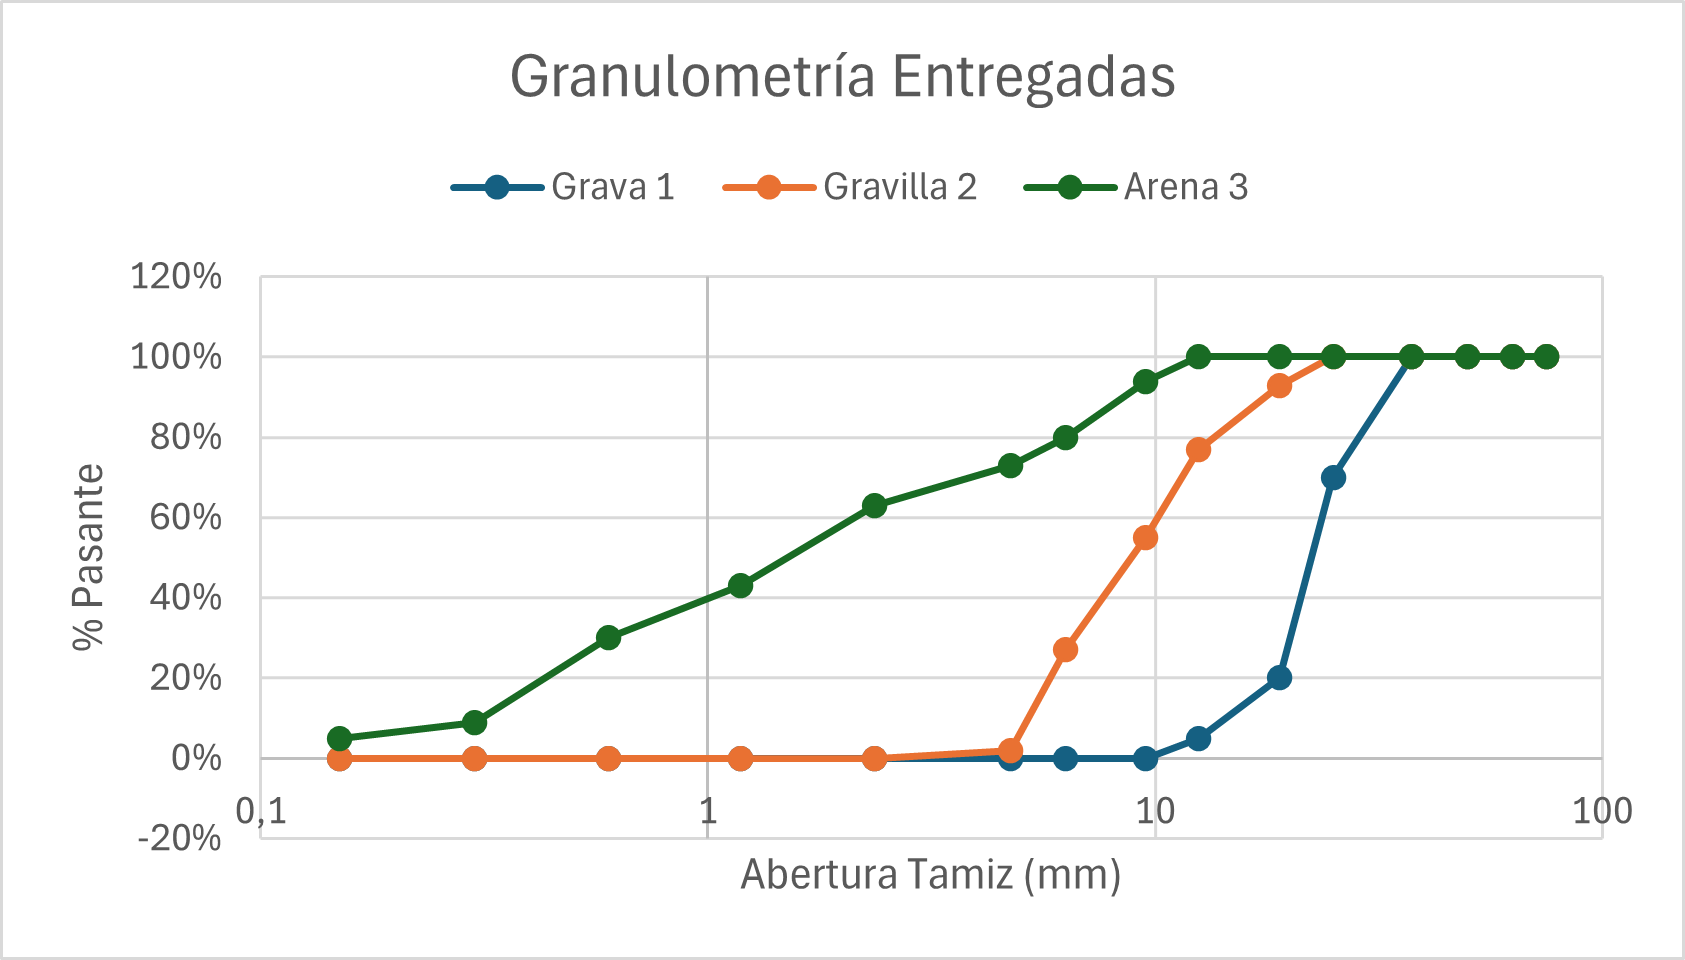
\includegraphics[width=0.8\textwidth]{GRAFICOS/granu_inicial.png}
    \caption{Curvas granulométricas de los áridos utilizados.}
    Fuente: Elaboración propia.
\end{figure}

Posteriormente, en base a la norma, se graficaron las curvas asociadas al $D_m = 10$ mm, ya que por condición inicial el TMA es 9,5 mm. Luego, se obtuvo la curva de granulometría sugerida, la cual es el promedio entre las curvas A, B, C y D. La figura se muestra a continuación.

\begin{figure}[H]
    \centering
    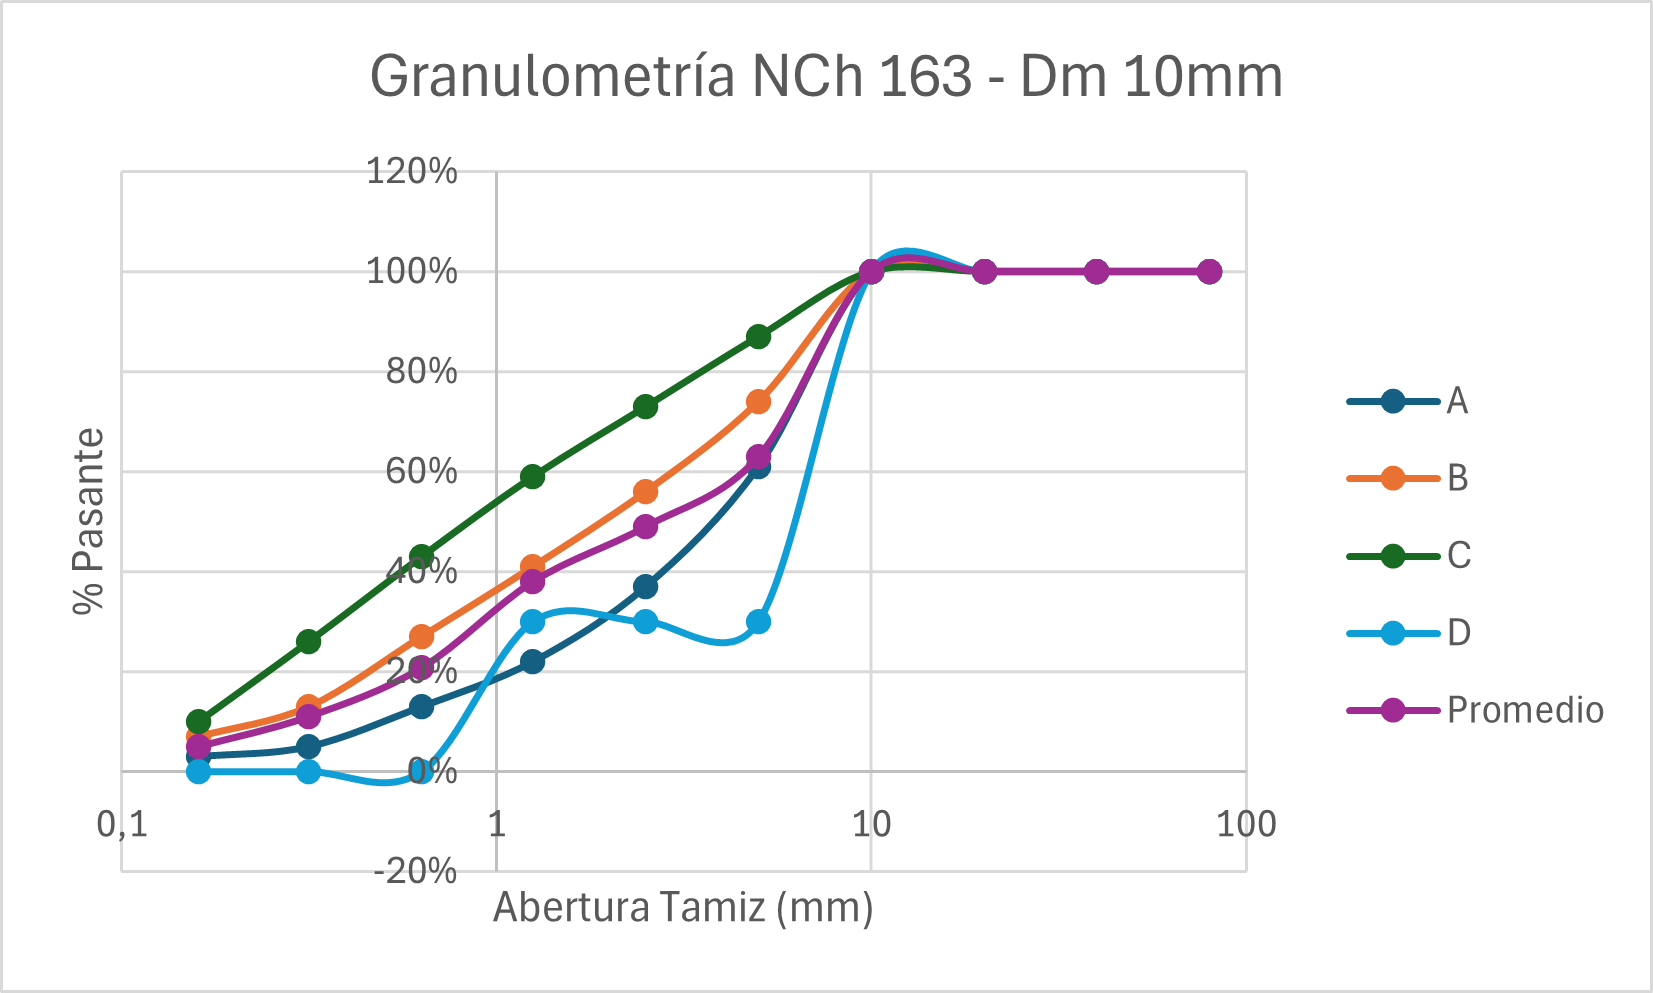
\includegraphics[width=0.8\textwidth]{GRAFICOS/NCh163.png}
    \caption{Curvas granulométricas de los áridos utilizados.}
    Fuente: Elaboración propia.
\end{figure}

Una vez obtenida la curva sugerida, se procede a la optimización granulométrica en base a la norma. Este proceso consistió en interpolar los porcentajes pasantes combinados de la mezcla inicial a los tamices indicados en la norma para poder compararlos. Finalmente, se realizó una iteración con la función objetivo de Excel para poder llevar la curva combinada a la sugerida, la cual varía los porcentajes de cada árido hasta que la diferencia entre ambas curvas sea igual a 0, manteniendo las condiciones y requerimientos iniciales, dando como resultado la curva optimizada.

La siguiente tabla muestra los porcentajes finales obtenidos para la ponderación de cada árido y la figura muestra la curva optimizada comparada con la curva sugerida. Se puede notar que la diferencia entre ambas está minimizada.

\begin{table}[H]
\centering
\caption{Ponderaciones finales de los áridos utilizando método de Banda.}
\begin{tabular}{|c|c|}
\hline
\textbf{Material} & \textbf{Ponderación Final (\%)} \\ \hline
Grava 1 & 19,02 \\ \hline
Gravilla 2 & 28,98 \\ \hline
Arena 3 & 51,99 \\ \hline
\end{tabular}
\\Fuente: Elaboración propia.
\end{table}

\begin{figure}[H]
    \centering
    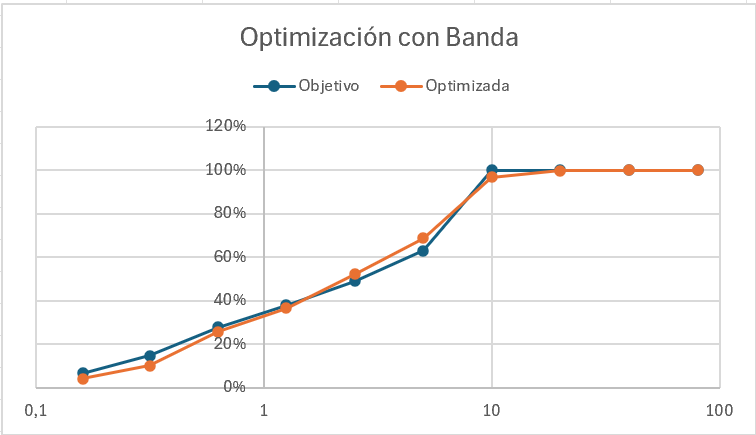
\includegraphics[width=0.8\textwidth]{GRAFICOS/opti_banda.png}
    \caption{Curva granulométrica optimizada comparada con la curva sugerida TMA.}
    Fuente: Elaboración propia.
\end{figure}

Además, siguiendo las normas y dadas las condiciones iniciales, las condiciones de ejecución en obra, el elemento a hormigonar, el tipo de hormigón y la clase de exposición en obra, se procedió a obtener el contenido de agua y cemento necesario para poder calcular el factor $K$, el cual corresponde a la masa total de áridos en estado SSS. Con estos datos, se pudo reemplazar en la ecuación de balance de volumen y obtener las proporciones finales de cada árido a utilizar en la mezcla optimizada.

\begin{table}[H]
\centering
\caption{Factor K y dosificación - TMA}
\label{tab:factor-k-tma}
\setlength{\tabcolsep}{6pt}
\renewcommand{\arraystretch}{1.15}
\small
\begin{tabular}{|l|r|c|}
\hline
\textbf{Volumen} & \textbf{1} & \textbf{m$^{3}$} \\ \hline
w          & 177,98     & kg/m$^{3}$ \\ \hline
c          & 286,14     & kg/m$^{3}$ \\ \hline
K          & 1933,09    & kg/m$^{3}$ \\ \hline
Grava 1    & 367,69     & kg/m$^{3}$ \\ \hline
Gravilla 2 & 560,24     & kg/m$^{3}$ \\ \hline
Arena 3    & 1005,15     & kg/m$^{3}$ \\ \hline
Aire       & 1,00       & \% \\ \hline
\end{tabular}
\\ Fuente: Elaboración propia.
\end{table}

Por último, obtenidas las proporciones finales de cada árido y la granulometría optimizada, se corrigió cada cantidad por humedad y rendimiento, obtuviendo los siguientes resultados.

\begin{table}[H]
\centering
\caption{Rendimiento de mezcla y factor de densidad}
\label{tab:rend-y-factor}
\small
\setlength{\tabcolsep}{6pt}
\renewcommand{\arraystretch}{1.15}

\begin{subtable}[t]{0.38\textwidth}
\centering
\caption{Densidades}
\label{tab:factor-rendimiento}
\begin{tabular}{lr}
\toprule
\textbf{Concepto} & \textbf{Valor} \\
\midrule
Densidad teórica & 2397,22 \\
Densidad real    & 2350 \\
Factor de densidad          & 0,9803 \\
\bottomrule
\end{tabular}
\\Fuente: Elaboración propia.
\end{subtable}
\begin{subtable}[t]{0.58\textwidth}
\centering
\caption{Corrección por Rendimiento TMA}
\label{tab:rendimiento}
\begin{tabular}{lrrr}
\toprule
 & \textbf{Teórico} & \textbf{Real} & \textbf{Corregida} \\
\midrule
Cemento   & 286,15 & 280,51 & 286,15 \\
Agua      & 82,86  & 81,23  & 82,86  \\
Agregados & 2028,22 & 1988,26 & 1980,99 \\
Densidad  & 2111,08 & 2350,00 & 2350,00 \\
\bottomrule
\end{tabular}
\\Fuente: Elaboración propia.
\end{subtable}


\end{table}


\begin{table}[H]
\centering
\caption{Corrección por humedad (TMA = 9{,}5 mm).}
\label{tab:correccion-humedad}
\setlength{\tabcolsep}{6pt}
\renewcommand{\arraystretch}{1.15}
\small
\makebox[\textwidth][c]{%
\begin{tabular}{@{} l c c c c c c @{}} 
\toprule
\textbf{Material} & 
\textbf{SSS (kg/m$^{3}$)} & 
\textbf{Absorción (\%)} &
\textbf{Agua absorción (kg/m$^{3}$)} & 
\textbf{Humedad (\%)} &
\textbf{Peso seco (kg/m$^{3}$)} & 
\textbf{Áridos húmedos (kg/m$^{3}$)} \\
\midrule
Cemento                 & 286,15 & --   & --         & --   & --       & 286,15 \\
Agua de amasado         & 177,98 & --   & --         & --   & --       & 82,86 \\
Agua de abs.\ de áridos & --     & --   & 23,28      & --   & --       & -23,28 \\
\midrule
Grava 1                 & 367,69 & 1,30 & -4,72      & 4,00 & 362,97   & 377,49 \\
Gravilla 2              & 560,25 & 1,20 & -6,64      & 8,00 & 553,61   & 597,89 \\
Arena 3                 & 1005,16& 1,20 & -11,92     & 6,00 & 993,24   & 1052,83 \\
Aire                    & --     & -- & --         & --   & --       & 1,00\%\\
\midrule
Peso hormigón (kg)      & 2397,23&      &            &      &          & 2397,23 \\
\bottomrule
\end{tabular}%
}
\\Fuente: Elaboración propia.
\end{table}


\subsection{Fuller - Thompson}

En esta sección se realizó una nueva optimización granulométrica utilizando el método de Fuller-Thompson. Esta curva sigue una distribución de potencia, como se expresa a continuación:

\begin{equation}
    P(D) = 100 \times \left( \frac{D}{D_{\text{max}}} \right)^n
\end{equation}

Donde \(P(D)\) es el \% que pasa por el tamiz de diámetro \(D\), \(D_{\text{max}}\) es el tamaño máximo del árido (TMA) y \(n\) es el exponente que define la forma de la curva, el cual, según Fuller, tiene un valor de 0,5 para hormigones.

El objetivo es lograr que la curva de los áridos combinados con los \% optimizados sea lo más parecida a la curva sugerida por el método Fuller - Thompson, minimizando su diferencia. La curva sugerida se obtiene reemplazando la dosificación sugerida por la NCH 163 en la fórmula anterior.  

A continuación se muestran los resultados obtenidos.

\begin{table}[H]
\centering
\caption{Ponderaciones finales de los áridos utilizando Fuller-Thompson.}
\begin{tabular}{|l|c|}
\hline
\textbf{Material} & \textbf{Ponderación Final (\%)} \\ \hline
Grava 1     & 19,20 \\ \hline
Gravilla 2  & 28,86 \\ \hline
Arena 3     & 51,94 \\ \hline
\end{tabular}
\end{table}

\begin{figure}[H]
    \centering
    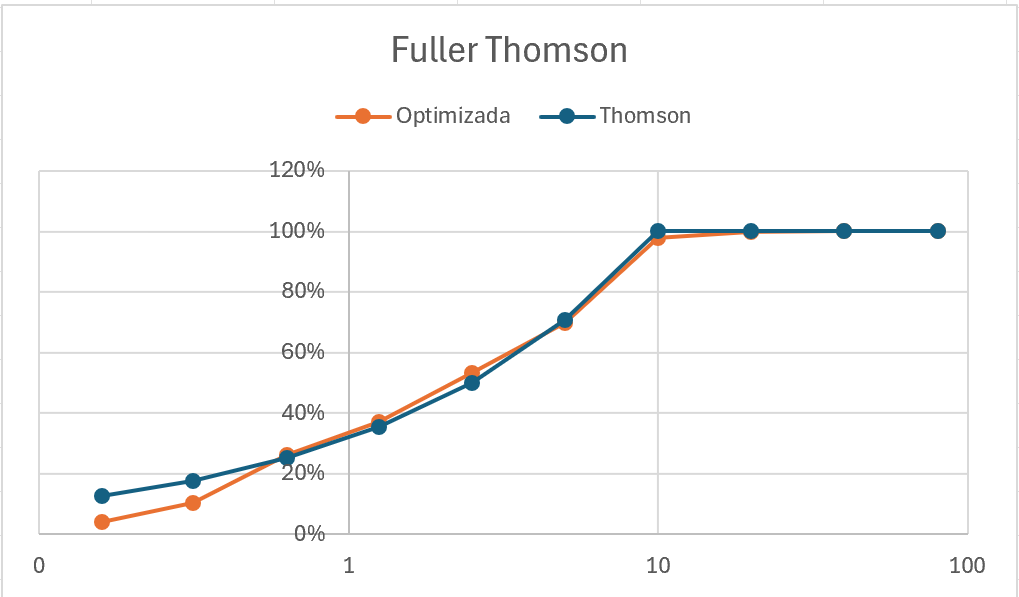
\includegraphics[width=0.8\textwidth]{GRAFICOS/fuller_thompson.png}
    \caption{Curva granulométrica optimizada por Fuller-Thompson.}
    Fuente: Elaboración propia.
\end{figure}

Se puede analizar que los resultados son similares a los obtenidos por el método de Banda, donde hay una cantidad similar de grava y gravilla con una dosis considerable de arena. Además, se puede observar que la diferencia de cada punto de la curva optimizada con la sugerida también es mínima. Las diferencias notorias se pueden ver más adelante, en el análisis de la curva Tarántula (Figura 5).

\begin{table}[H]
\centering
\caption{Factor K Fuller--Thompson}
\label{tab:factor-k-thomson}
\setlength{\tabcolsep}{6pt}
\renewcommand{\arraystretch}{1.15}
\small
\begin{tabular}{|l|r|c|}
\hline
\textbf{Volumen} & \textbf{1,000000} & \textbf{m$^{3}$} \\ \hline
w          & 177,98     & kg/m$^{3}$ \\ \hline
c          & 286,15     & kg/m$^{3}$ \\ \hline
k          & 1923,12    & kg/m$^{3}$ \\ \hline
Grava 1    & 369,20     & kg/m$^{3}$ \\ \hline
Gravilla 2 & 555,09     & kg/m$^{3}$ \\ \hline
Arena 3    & 998,84     & kg/m$^{3}$ \\ \hline
Aire & 1,00 & \% \\ \hline
\end{tabular}
\\ Fuente: Elaboración propia.
\end{table}

Posteriormente, se obtuvieron las masas requeridas de agua, cemento y agregados corregidas, utilizando las
condiciones y requerimientos iniciales.

\begin{table}[H]
\centering
\caption{Rendimiento Fuller-Thompson y factor de densidad}
\label{tab:rendimiento-factor-thomson}
\small
\setlength{\tabcolsep}{6pt}
\renewcommand{\arraystretch}{1.15}
\begin{subtable}[t]{0.38\textwidth}
\centering
\caption{Densidades}
\begin{tabular}{lr}
\toprule
\textbf{Concepto} & \textbf{Valor} \\
\midrule
Densidad teórica & 2387,25 \\
Densidad real    & 2350 \\
Factor           & 0,9844 \\
\bottomrule
\end{tabular}
\\ Fuente: Elaboración propia.
\end{subtable}
\hfill
\begin{subtable}[t]{0.58\textwidth}
\centering
\caption{Corrección por Rendimiento F--T}
\setlength{\tabcolsep}{6pt}
\renewcommand{\arraystretch}{1.15}
\small
\begin{tabular}{lrrr}
\toprule
 & \textbf{Teórico} & \textbf{Real} & \textbf{Corregida} \\
\midrule
Cemento   & 286,14 & 281,68 & 286,14 \\
Agua      & 83,47  & 82,17  & 83,47  \\
Agregados & 2017,64 & 1986,15 & 1980,38 \\
Densidad  & 2387,25 & 2350   & 2350   \\
\bottomrule
\end{tabular}
\\Fuente: Elaboración propia.
\end{subtable}
\end{table}

\begin{table}[H]
\centering
\captionsetup{justification=centering}
\caption{Corrección por humedad y dosificación Fuller-Thompson.}
\label{tab:correccion-humedad-thomson}
\setlength{\tabcolsep}{6pt}
\renewcommand{\arraystretch}{1.15}
\small
\makebox[\textwidth][c]{%
\begin{tabular}{@{} l r r r r r @{}} % l + 5 numéricas
\toprule
\textbf{Material} &
\textbf{SSS (kg/m$^{3}$)} &
\textbf{Agua absorción (kg/m$^{3}$)} &
\textbf{Peso seco (kg/m$^{3}$)} &
\textbf{Agua total (kg/m$^{3}$)} &
\textbf{Áridos húmedos (kg/m$^{3}$)} \\
\midrule
Cemento                 & 286,15 & --      & --      & --        & 286,15 \\
Agua de amasado         & 177,98 & --      & --      & -23,16    & 83,47  \\
Agua de abs.\ de áridos & --     & 23,16   & --      & -117,68   & --     \\
\midrule
Grava 1                 & 369,20 & -4,74   & 364,46  & 14,58     & 379,04 \\
Gravilla 2              & 555,09 & -6,58   & 548,51  & 43,88     & 592,39 \\
Arena 3                 & 998,84 & -11,84  & 986,99  & 59,22     & 1046,21 \\
Aire                    &   --    &    --       &  --        &    --    & 1,00\% \\
\midrule
\textbf{Peso hormigón (kg)} & \textbf{2387,26} &  &  &  & \textbf{2387,26} \\
\bottomrule
\end{tabular}%
}
\\Fuente: Elaboración propia.
\end{table}


\subsection{Curva Tarántula}

En esta sección se analizarán los resultados obtenidos utilizando el método de la Curva Tarántula para evaluar su trabajabilidad. Es importante mencionar que las proporciones finales de cada árido en cada método de optimización fueron ajustadas para que cumplieran las condiciones de la Curva Tarántula.

En primer lugar, con las diferentes fracciones de las partículas y con los datos iniciales, se calculó el porcentaje pasante acumulado para cada tamiz, lo que permitió construir la Curva Tarántula. Esta curva se comparó con los límites superior e inferior establecidos por la norma, lo que asegura que la mezcla de áridos cumpla con los requisitos de estabilidad y trabajabilidad.

Se aplicaron los métodos TMA y Fuller-Thompson para ajustar la distribución granulométrica de la mezcla, optimizando la proporción de cada tipo de árido. Posteriormente, se verificó que la mezcla ajustada cumpliera con los criterios de la Curva Tarántula.

Finalmente, se generó un gráfico comparativo entre las curvas de TMA, Fuller-Thompson y los límites de la Curva Tarántula. Este proceso garantiza la adecuada formulación de la mezcla de hormigón para una buena trabajabilidad y estabilidad.

\begin{figure}[H]
    \centering
    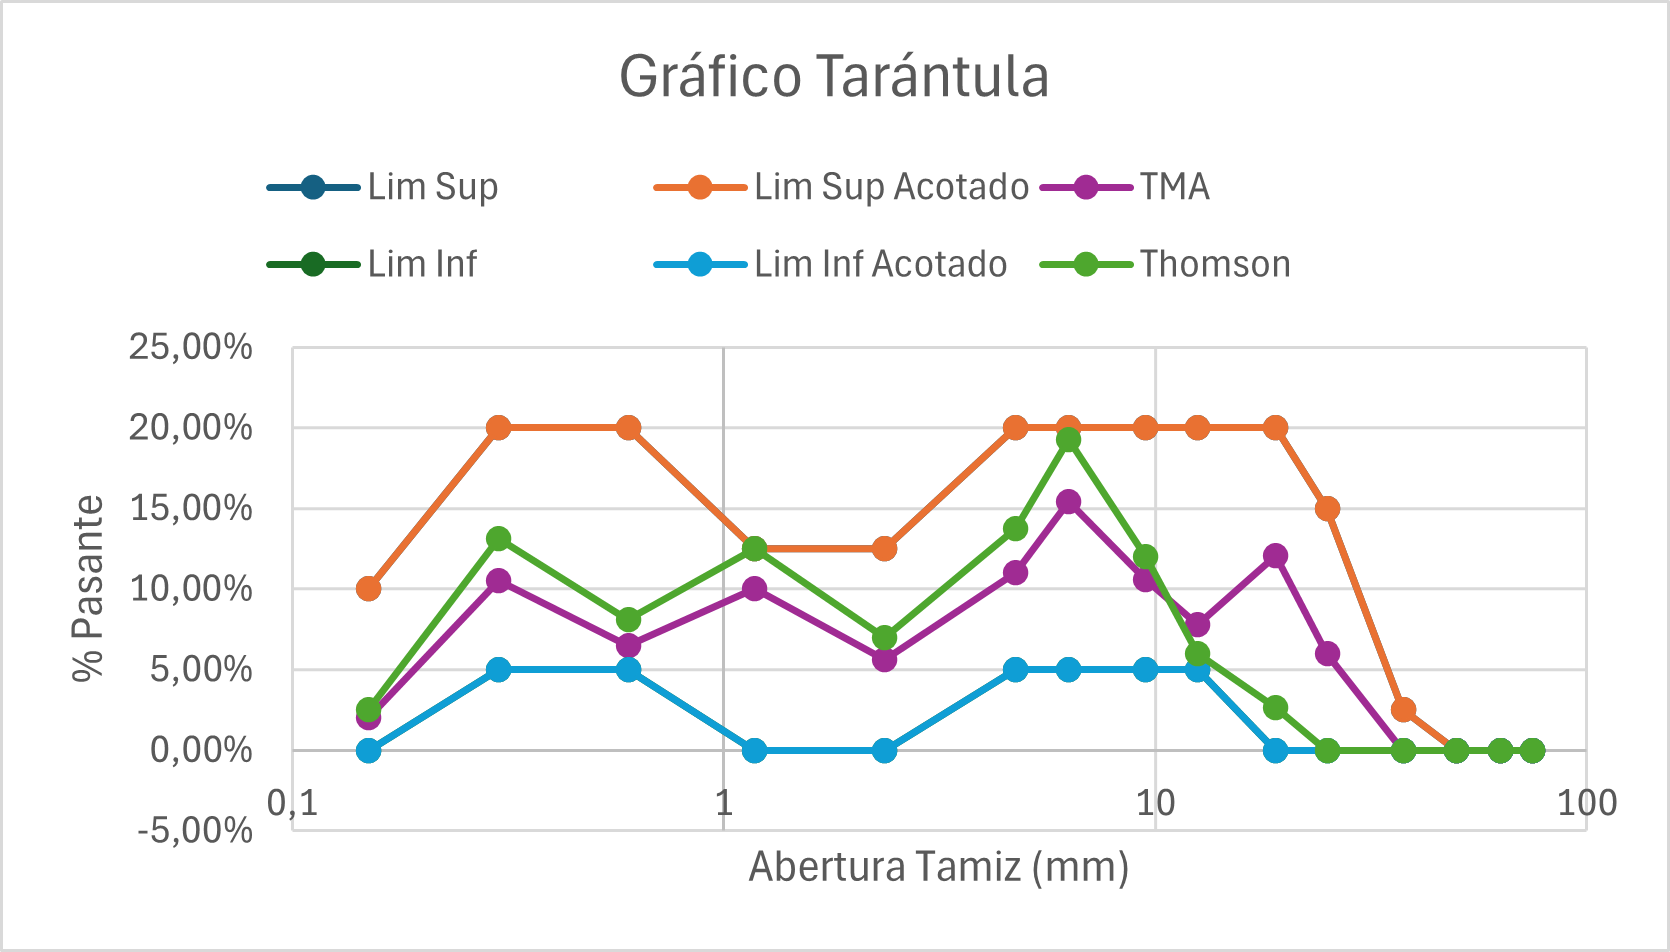
\includegraphics[width=0.8\textwidth]{GRAFICOS/tarantula.png}
    \caption{Comparación de curvas de TMA, Fuller-Thompson y límites de la Curva Tarántula.}
    \label{fig:curva_tarantula}
    Fuente: Elaboración propia.
\end{figure}

\begin{table}[H]
\centering
\caption{Comparación de dosificación final y porcentaje de diferencia entre TMA y Fuller-Thompson.}
\label{tab:comparacion-dosificacion}
\begin{tabular}{|l|c|c|c|}
\hline
\textbf{Material} & \textbf{Dosificación Final (TMA) (kg)} & \textbf{Dosificación Final (Fuller) (kg)} & \textbf{Diferencia (\%)} \\ \hline
Cemento           & 286,14                               & 286,14                                & 0\%                     \\ \hline
Agua de amasado   & 86,83                                & 86,83                                 & 0\%                     \\ \hline
Grava 1           & 517,82                               & 567,71                                & -8,77\%                 \\ \hline
Gravilla 2        & 513,36                               & 477,42                                & +7,54\%                 \\ \hline
Arena 3           & 983,41                               & 983,41                                & 0\%                     \\ \hline
Aire              & 1,00\%                               & 1,00\%                                & 0\%                     \\ \hline
Peso Hormigón     & 2406,41                              & 2406,34                               & 0,03\%                  \\ \hline
\end{tabular}
\end{table}

El gráfico compara las curvas combinadas de TMA y Fuller-Thompson con los límites de la Curva Tarántula para TMA = 9,5 mm. Ambas mezclas se mantienen dentro del rango aceptable, lo que indica una buena trabajabilidad y estabilidad.

En la fracción de finos (\(<0,3~\text{mm}\)), las curvas evitan el déficit de finos y el exceso de partículas finas, lo que favorece una pasta trabajable. En el rango de arena gruesa (\(0,6-2,36~\text{mm}\)), el control de partículas mejora el deslizamiento y estabiliza el asentamiento. Los áridos gruesos (\(2,36-4,75~\text{mm}\)) presentan una distribución adecuada sin generar vacíos intermedios.

La curva Fuller-Thompson es levemente más fina en la zona de finos, mientras que la curva TMA se ajusta bien en el rango de \(2,36-4,75~\text{mm}\). Ambas metodologías son válidas y su selección depende de la disponibilidad de áridos y las pruebas de mezcla.

En resumen, ambas curvas cumplen con la Curva Tarántula, con buen desempeño en la fracción de arena gruesa, lo que asegura una mezcla cohesiva y bombeable.

Para finalizar, se presenta el gráfico comparativo entre la curva optimizada por Banda, Fuller-Thompson y las granulometrías iniciales.

\begin{figure}[H]
    \centering
    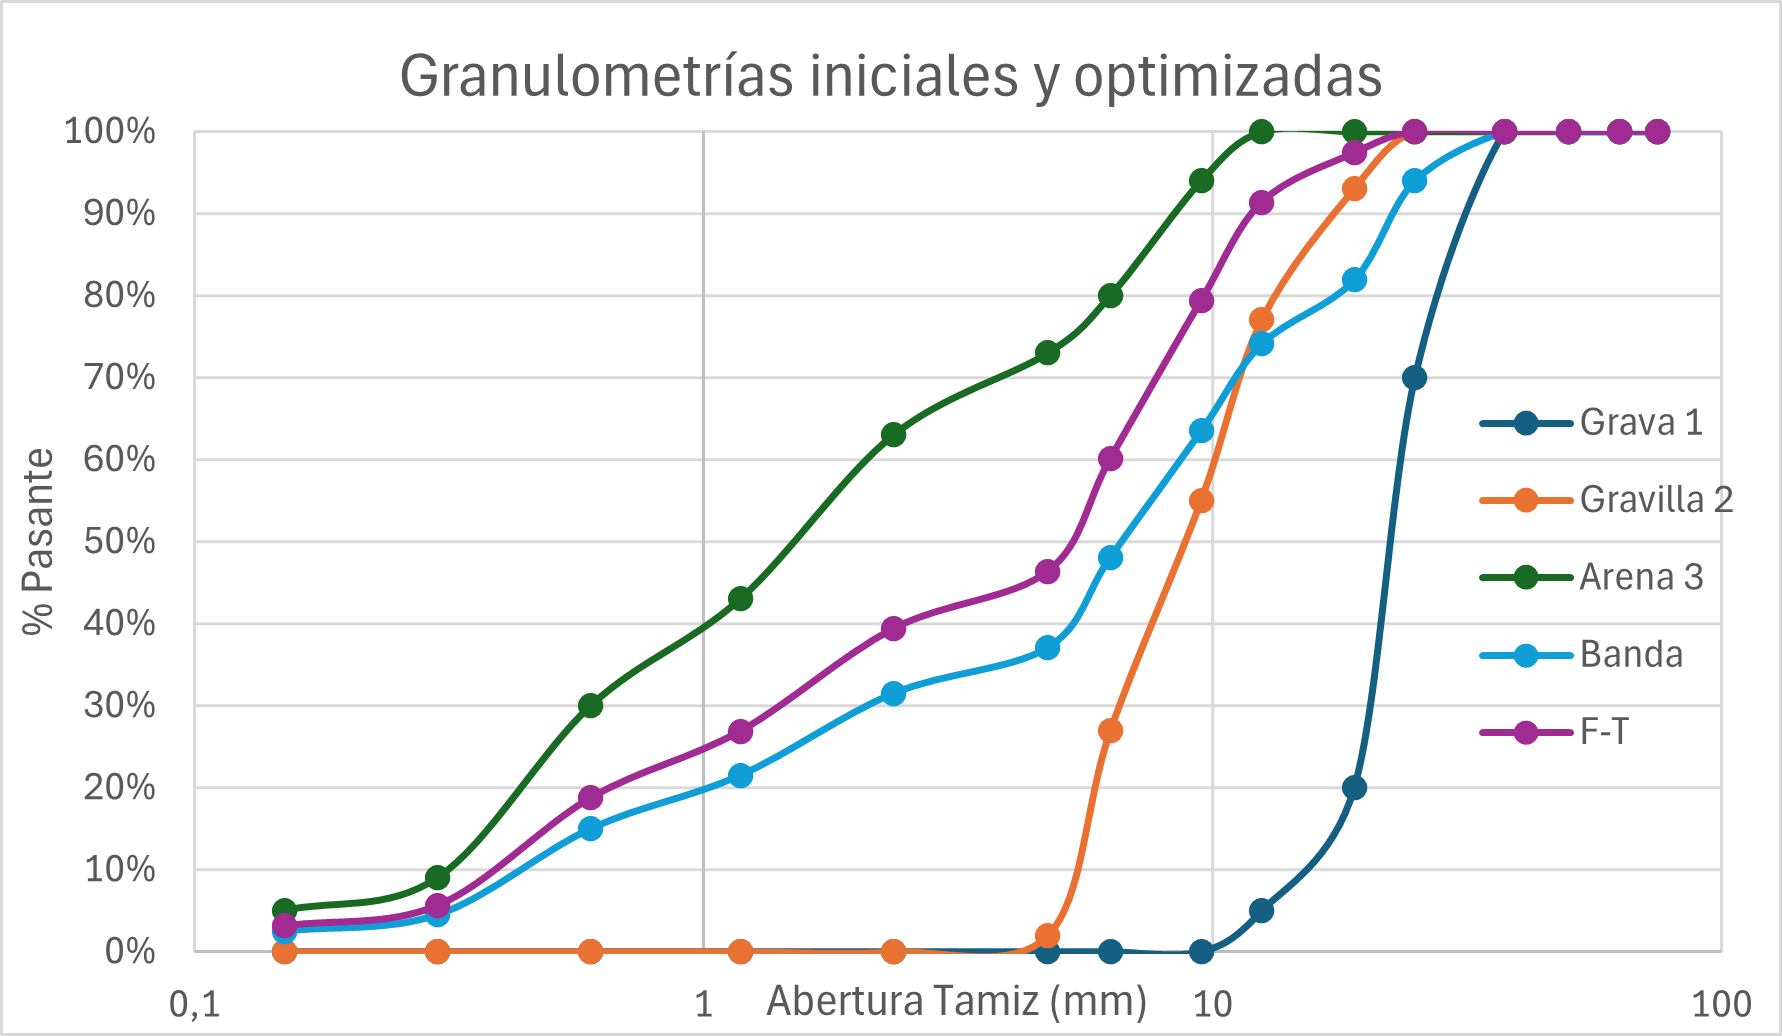
\includegraphics[width=0.8\textwidth]{GRAFICOS/granu_final.png}
    \caption{Comparación de curvas optimizadas por Banda, Fuller-Thompson y granulometrías iniciales.}
    \label{fig:curvas_comparativas}
    Fuente: Elaboración propia.
\end{figure}

\subsection{Discusión}

\subsubsection*{i)}

El método del ACI 211.1-22 entrega una dosificación inicial basada en relaciones empíricas entre asentamiento, tamaño máximo de árido y resistencia especificada, proporcionando un procedimiento estandarizado y ampliamente validado \cite{ACI211.1-22}. En cambio, la curva Tarántula busca optimizar la granulometría de los áridos mediante un ajuste fino de la distribución, con el fin de reducir vacíos, mejorar la compactación y lograr una mezcla más densa \cite{Beltran2024TarantulaCurve}. Las diferencias observadas radican en que el método ACI puede generar mezclas con mayor consumo de pasta, mientras que la curva Tarántula promueve una reducción en el contenido de pasta gracias a una mejor gradación. Para el caso específico analizado, la curva Tarántula se recomienda cuando se busca optimizar costos y reducir retracciones, siempre y cuando se disponga de un control detallado de la granulometría de los áridos.

\subsubsection*{ii)}

Los materiales cementicios suplementarios (SCM) cumplen un rol clave en la mejora de la durabilidad, la sustentabilidad y el desempeño mecánico del hormigón. Entre ellos se incluyen las cenizas volantes, escorias granuladas de alto horno y puzolanas naturales, que permiten reemplazar parcialmente al cemento, reduciendo las emisiones de CO$_2$ asociadas a su producción y optimizando la resistencia frente a agentes agresivos. \cite{ScienceDirect_SCMs}

En este caso, se incorporó un 30\% de reemplazo de cemento por ceniza volante de tipo F (Fly Ash), una puzolana de carácter silíceo y alumínico que reacciona lentamente con la cal liberada durante la hidratación. Esta elección se justifica porque la mezcla está destinada a un ambiente moderado, en el cual la adición de ceniza volante contribuye a mejorar la trabajabilidad en estado fresco, disminuir el calor de hidratación y densificar la microestructura de la pasta, reduciendo su permeabilidad. 

\begin{table}[H]
\centering
\caption{Dosificación comparativa con y sin ceniza volante tipo F (valores corregidos por rendimiento).}
\label{tab:comp-dosificacion-fa}
\setlength{\tabcolsep}{6pt}
\renewcommand{\arraystretch}{1.15}
\small
\makebox[\textwidth][c]{%
\begin{tabular}{@{} l c c c c c c @{}} % columnas centradas
\toprule
\textbf{Caso} & \textbf{Cemento} & \textbf{Fly Ash} & \textbf{Agua} & \textbf{Agregados} & \textbf{Densidad} & \textbf{Relaciones} \\
 & \textbf{(kg/m$^{3}$)} & \textbf{(kg/m$^{3}$)} & \textbf{(kg/m$^{3}$)} & \textbf{(kg/m$^{3}$)} & \textbf{(kg/m$^{3}$)} & \textbf{$w/c$ \;|\; $w/(c{+}FA)$} \\
\midrule
Con FA (30\%) & 200{,}30 & 60{,}09 & 82{,}89 & 2066{,}83 & 2350 & 0{,}414 \;|\; 0{,}318 \\
Sin SCM           & 286{,}15 & 0{,}00  & 83{,}47 & 1980{,}50 & 2350 & 0{,}292 \;|\; --- \\
\bottomrule
\end{tabular}%
}
\\Fuente: Elaboración propia.
\end{table}

La incorporación de ceniza volante tipo F como material cementicio suplementario (30\% del cemento) refina la microestructura de la pasta, disminuye la permeabilidad y la exudación, y reduce el calor de hidratación. Sin embargo, el desarrollo resistente temprano puede ser más lento. Dado que cambia el reparto de la matriz, es más representativo controlar la razón $w/(c+FA)$ que sólo $w/c$. En la práctica, el efecto reológico de la ceniza permite reducir el agua en torno a un 3–5\% para conservar el asentamiento objetivo y optimizar la relación agua–cemento sin perder cohesión.

Respecto de la curva Tarántula, la sustitución de cemento por ceniza no altera la granulometría de los áridos, por lo que los pasantes y el cumplimiento de límites se mantienen invariables. En trabajabilidad, con igual agua se espera una fluidez mayor y menor tendencia a segregación de las partículas de ceniza. También, se puede mantener el mismo asentamiento con menos agua, mejorando $w/(c+FA)$ y la bombeabilidad sin afectar el diseño granulométrico ni el TMA.


\subsubsection*{iii)}

La curva de Fuller-Thomson busca una distribución continua ideal para maximizar la densidad del empaquetamiento de los áridos \cite{Vidal2025FullerThompson}. La banda granulométrica según TMA (tamaño máximo del árido) entrega un rango de aceptación más amplio, sin perseguir necesariamente la densidad máxima \cite{NCh1632013}. Cuando existe una diferencia significativa, puede generarse mayor consumo de pasta para rellenar vacíos, afectando costos y retracción. Una solución es ajustar la dosificación de finos, de modo que la curva real se acerque al mismo tiempo a ambos criterios.

\subsubsection*{iv)}

Si la mezcla se diseña con la mitad del agua, la trabajabilidad se vería comprometida. En este caso, la normativa \cite{ACI211_2022}, \cite{ACI301_2020} y \cite{NCh1632013} recomienda el uso de aditivos reductores de agua o superplastificantes de alto rango (HRWR). Estos aditivos permiten mantener la relación w/c baja para garantizar alta resistencia, sin sacrificar trabajabilidad. El procedimiento de cálculo del aditivo se basa en el porcentaje de reducción de agua necesario, el cual puede variar entre 15\% y 30\% para aditivos reductores convencionales y hasta 40\% para HRWR. Al aplicarlo, la dosificación ajustada mantiene el contenido de agua equivalente al método original, logrando así un equilibrio entre resistencia y manejabilidad.

\subsubsection*{v)}

La humedad superficial y la absorción de los áridos influyen directamente en el agua efectiva de la mezcla. Si no se corrigen, se produce un error en la relación a/c, lo que impacta resistencia y trabajabilidad. En climas cálidos y secos (ejemplo: norte de Chile), la rápida evaporación reduce la trabajabilidad y puede provocar fisuración plástica, por lo que se recomienda prehumectar los áridos y utilizar retardadores de fraguado. En climas fríos y húmedos (ejemplo: zona sur), el riesgo se relaciona con ciclos de hielo-deshielo, donde se requiere aire incorporado para preservar la durabilidad. De esta forma, las correcciones por humedad y absorción deben ser consideradas en toda dosificación práctica, ajustando la mezcla en obra según condiciones locales.

\subsubsection*{vi)}

En la práctica, el rendimiento del hormigón difiere del teórico debido a variaciones en la densidad de los materiales. En el caso planteado, la densidad real fue de 2350 kg/m\(^3\) frente a una teórica de 2400 kg/m\(^3\).
\begin{enumerate}
    \item Estas diferencias se deben a variabilidad en los áridos, contenido de aire y compactación real en obra.
    \item El desajuste afecta el rendimiento porque se produce un mayor volumen por m\(^3\) de materiales, pudiendo generar déficit de mezcla y afectar la homogeneidad estructural.
    \item Aplicando el factor de corrección, se recalculan las cantidades de materiales para que el volumen total corresponda a 1 m\(^3\) de hormigón real, ajustando cemento, agua y áridos proporcionalmente.
    \item Este ajuste por rendimiento también influye en resistencia y durabilidad: un exceso de volumen sin ajuste puede generar menor densidad aparente, más porosidad y reducción de propiedades mecánicas a largo plazo.
\end{enumerate}
